\documentclass[11pt,twoside]{article}
\usepackage[T1]{fontenc}
\usepackage[latin1]{inputenc}
\usepackage[english]{babel}
\usepackage{amsmath}
\usepackage{amscd}
\usepackage{amssymb}
\usepackage{multirow}
\usepackage{tabularx}
\usepackage{url}
\usepackage{fancyhdr}
\usepackage{lastpage}
\usepackage{graphicx}
\usepackage[a4paper,margin=2.5cm,hmarginratio=1:1]{geometry}

%%%%%%%%%%%%%%%%%%%%%%%%%%%%%%%%%%%%%%%%%%%%%%%%%%%%%%%%%%%%%%%%%%%%%%%%%%%
%%%%%%%%%%%%%% ENTER YOUR PERSONAL INFORMATION HERE %%%%%%%%%%%%%%%%%%%%%%%
%%%%%%%%%%%%%%%%%%%%%%%%%%%%%%%%%%%%%%%%%%%%%%%%%%%%%%%%%%%%%%%%%%%%%%%%%%%


% Your name, personal number, and email.
\newcommand{\firstname}{Bastian}
\newcommand{\lastnames}{Fredriksson}
\newcommand{\persnr}{9302164216}
\newcommand{\email}{bastianf@kth.se}


% Your two study pals. Leave empty as necessary.
\newcommand{\studypalX}{}
\newcommand{\studypalXemail}{}


%%%%%%%%%%%%%%%%%%%%%%%%%%%%%%%%%%%%%%%%%%%%%%%%%%%%%%%%%%%%%%%%%%%%%%%%%%%
%%%%%%%%%%%%% DO NOT TOUCH ANYTHING BELOW THIS LINE %%%%%%%%%%%%%%%%%%%%%%%
%%%%%%%%%%%%%%%%%%%%%%%%%%%%%%%%%%%%%%%%%%%%%%%%%%%%%%%%%%%%%%%%%%%%%%%%%%%

\newcounter{problem}
\renewcommand\theproblem{\arabic{problem}}
\newenvironment{problem}{%
  \bigbreak
  \refstepcounter{problem}\noindent
  \llap{\textbf{\theproblem}\quad}\ignorespaces
}{%
  \par\if@nadaten@solutions\relax\else\filbreak\fi
}
\newenvironment{problem*}{%
  \bigbreak
  \refstepcounter{problem}\noindent
  \llap{\textbf{\theproblem}\quad}\ignorespaces
}{%
  \par
}
\newcounter{subproblem}[problem]
\renewcommand{\thesubproblem}{\arabic{problem}\alph{subproblem}}
\newenvironment{subproblem}{%
  \refstepcounter{subproblem}%
  \list{}{}%
  \item\leavevmode
  \llap{\hbox to \leftmargini{\textbf{\thesubproblem}\hfil}}%
  \ignorespaces
}{%
  \endlist\if@nadaten@solutions\relax\else\filbreak\fi
}
\newenvironment{subproblem*}{%
  \refstepcounter{subproblem}%
  \list{}{}%
  \item\leavevmode
  \llap{\hbox to \leftmargini{\textbf{\thesubproblem}\hfil}}%
  \ignorespaces
}{%
  \endlist
}

\newcommand{\homeworknr}{2}
\newcommand{\studentname}{\firstname~\lastnames}
\newcommand{\homework}{Homework~\homeworknr}
\newcommand{\coursenumber}{DD2448}
\newcommand{\coursename}{\coursenumber~Foundations of cryptography}
\newcommand{\coursenick}{krypto15}

\lhead[\studentname]{\coursename}
\chead{}
\rhead[\coursename]{\studentname}
\lfoot[\thepage~(\pageref{LastPage})]{}
\cfoot{}
\rfoot[]{\thepage~(\pageref{LastPage})}

\fancypagestyle{firststyle}
{
   \fancyhf{}
   \fancyfoot[R]{\thepage~(\pageref{LastPage})}
}

\renewcommand{\headrulewidth}{0pt}


%%%%%%%%%%%%%%%%%%%%%%%%%%%%%%%%%%%%%%%%%%%%%%%%%%%%%%%%%%%%%%%%%%%%%%%%%%%
%%% HERE YOU CAN ADD YOUR OWN MACROS AND ENVIRONMENTS IN THE PREAMBLE %%%%%
%%%%%%%%%%%%%%%%%%%%%%%%%%%%%%%%%%%%%%%%%%%%%%%%%%%%%%%%%%%%%%%%%%%%%%%%%%%

% Add your macros here.


\begin{document}

%%%%%%%%%%%%%%%%%%%%%%%%%%%%%%%%%%%%%%%%%%%%%%%%%%%%%%%%%%%%%%%%%%%%%%%%%%%
%%%%%%%%%%%% THE FOLLOWING GENERATES THE HEADER %%%%%%%%%%%%%%%%%%%%%%%%%%%
%%%%%%%%%%%% DO NOT TOUCH THIS %%%%%%%%%%%%%%%%%%%%%%%%%%%%%%%%%%%%%%%%%%%%
%%%%%%%%%%%%%%%%%%%%%%%%%%%%%%%%%%%%%%%%%%%%%%%%%%%%%%%%%%%%%%%%%%%%%%%%%%%

\thispagestyle{firststyle}

\noindent
\hspace{0.3cm}{\huge\textbf{\coursename}}

\noindent
\rule{\textwidth}{1pt}

\vspace{0.3cm}

\noindent
\begin{tabularx}{\textwidth}{lXl}
  \multirow{3}{*}{\textbf{\huge\homework}} && {\Large\textbf{\studentname}} \\
&&\\[-0.3cm]
  && {\Large\persnr} \\
&&\\[-0.35cm]
  && {\Large\texttt{\email}} \\
&&\\[-0.2cm]
\cline{3-3}
&&\\[-0.2cm]
  \multirow{2}{*}{\textbf{\huge\coursenick}} && {\small\studypalX, \texttt{\studypalXemail}} \\
&& {\small\studypalY, \texttt{\studypalYemail}}
\end{tabularx}

\vspace{0.2cm}
\noindent
\rule{\textwidth}{1pt}

\vspace{0.5cm}

\pagestyle{fancy}

%%%%%%%%%%%%%%%%%%%%%%%%%%%%%%%%%%%%%%%%%%%%%%%%%%%%%%%%%%%%%%%%%%%%%%%%%%%
%%%%%%%%%%%%%%%%%%%%% YOUR SOLUTIONS START HERE %%%%%%%%%%%%%%%%%%%%%%%%%%%
%%%%%%%%%%%%%%%%%%%%%%%%%%%%%%%%%%%%%%%%%%%%%%%%%%%%%%%%%%%%%%%%%%%%%%%%%%%
%%                                                                       %%
%%  Do NOT remove any problem-, or subproblem environments below. If     %%
%%  you can not solve a problem, then you MUST simply leave the "NOT     %%
%%  SOLVED" string intact. This ensures that the numbering is correct    %%
%%  and it simplifies grading, leaving more time to prepare lectures     %%
%%  and help students.                                                   %%
%%                                                                       %%
%%  Do not remove any point markers. Leaving them in place simplifies    %%
%%  grading.                                                             %%
%%                                                                       %%
%%%%%%%%%%%%%%%%%%%%%%%%%%%%%%%%%%%%%%%%%%%%%%%%%%%%%%%%%%%%%%%%%%%%%%%%%%%

\begin{problem}
  (3I) IMPLEMENTED
\end{problem}

\begin{problem}
  (3I) IMPLEMENTED
\end{problem}

\begin{problem}
  (5I) IMPLEMENTED
\end{problem}

\begin{problem}
  (2I) NOT SOLVED % Elliptiska kurvor
\end{problem}

\begin{problem}
  (8T) % SSL-TLS
  SSL (Secure Sockets Layer) and TLS (Transport Layer Security) are \textit{cryptographic protocols} used to secure a connection between a client and a server. SSL and TLS and typically used together with HTTP, so called HTTPS-connections. Thus, SSL/TLS are widely used as a way of \textit{secure web browsing}. This is important when you send information like credit card numbers, passwords and other private information to a bank or a web shop. But SSL/TLS is also used in IM programs, VOIP services and for sending emails. 
  
  The first widely used protocol was SSLv2, which was invented by Netscape in 1995. SSLv2 contained some severe security bugs which were patched in 1996 when SSLv3 was released. The security vulnerabilities of SSlv2 included the use of MD5 as MAC algorithm, no protection against MitM-attacks and the same key was used for both message authentication and encryption. The reason why MD5 is not a good choice for message authentication is because it is (practically) possible to create collisions. 
  
  SSLv3 was considered secure until 2011 when the POODLE attack (Padding Oracle On Downgraded Legacy Encryption) was discovered. POODLE exploited a weakness in the SSLv3 protocol and allowed an attacker to mount a MitM-attack and decrypt ciphertext using a side-channel attack. Although a POODLE-attack is difficult to perform in practice, SSLv3 is not considered secure and should not be used. 
  
  TLSv1.0 came in 1999 as an upgrade of SSLv3 and is still in use in many clients (e.g Postfix, Asterisk and older web browsers). TLSv1.0 added support for ciphers based on Elliptic Curve cryptography but it was still backward compatible with SSLv3 in the sense that clients who did not support TLSv1.0 were allowed to use SSLv3. TLSv1.0 also came with an option called TLS\_FALLBACK\_SCSV. This is a flag which allows the client to report to the server which protocols it supports. If the client tries to downgrade to an older protocol once a connection has been established, the server closes the connection (downgrade attack prevention). This makes it impossible for an attacker to force the server to use a less secure protocol once the handshake is completed. 
  
  TLSv1.1 was released in 2006 and TLSv1.2 was released in 2008. Although all modern browsers support TLSv1.2, adaption has been meagre and many mail client ect still uses TLSv1.0. TLSv1.1 and newer contains fixes for attacks with funny abbreviations like CRIME and BEAST. CRIME (Compression Ratio Info-leak Made Easy) allowed an attacker to recover authentication cookies and hijack an HTTPS-session. This is only possible if the client-server connection uses data compression, so the easy fix is to disable this option server-side. 
  
  BEAST exploits a security flaw in TLSv1.0 which allows an attacker to predict the IV (initialisation vector) used to mask data prior to encryption when utilising AES in block cipher mode of operation (AES-CBC). If an attacker is can see and change the data sent between server and client (e.g mount a MitM-attack), he'll be able to make guesses about the plaintext. In pratice, this would allow an attacker to recover small parts of the plaintext, like cookies. At the time BEAST was discovered the only way of mitigating it (server-side) was to enable ciphers suites which included the RC4 stream cipher. However, at about this time, researchers found that RC4 was much weaker than previously expected and the recommendation became to disable RC4, thus opening up for the BEAST attack. Since BEAST was a client-side issue, most browsers (except Apples Safari) were quite quick to implement a fix. Currently, most browsers (including Safari) mitigates BEAST, so the recommendation is to leave RC4 off. Modern cipher suites utilises AES-GCM which is not vulnerable to BEAST.
  
  TLS/SSL uses certificates to verify the identity of a server. An certificate signing request (CSR) contains information about the owner, which domain the certificate is valid for, an the date of expiry ect. The content of the CRT is \textit{signed} by a Certificate Authority (CA). A certificate presented to a client includes both the content of the CSR (certificate) and a hash encrypted with the CA:s private key. The client verifies the identity by verifying (decrypting) the signature presented by the server and compare it with a hash of the certificate. The private-public cryptosystem used the verify and create signatures is RSA with at least 2048 bit key size (shorter keys are no longer accepted by some clients). 
  
  This system is flawed in many ways. What if someone steal the CA:s private key? This happened for DigiNotar in 2011, which issued certificates for the Dutch government. During the latest month, companies like Google have made changes to their Chrome web browser starting to warn users about (some) sites using certificates signed with SHA1. The reason is that it might be possible to find collisions in SHA1 and forge certificates by 2020 (or maybe as early as 2018, depending on your budget). However, many CA:s still issues certificates signed with SHA1 and users who have been paying for a certificate are reluctant to pay for yet another one.
\end{problem}

\begin{problem}
  \begin{subproblem}
  \begin{figure}
    \centering
    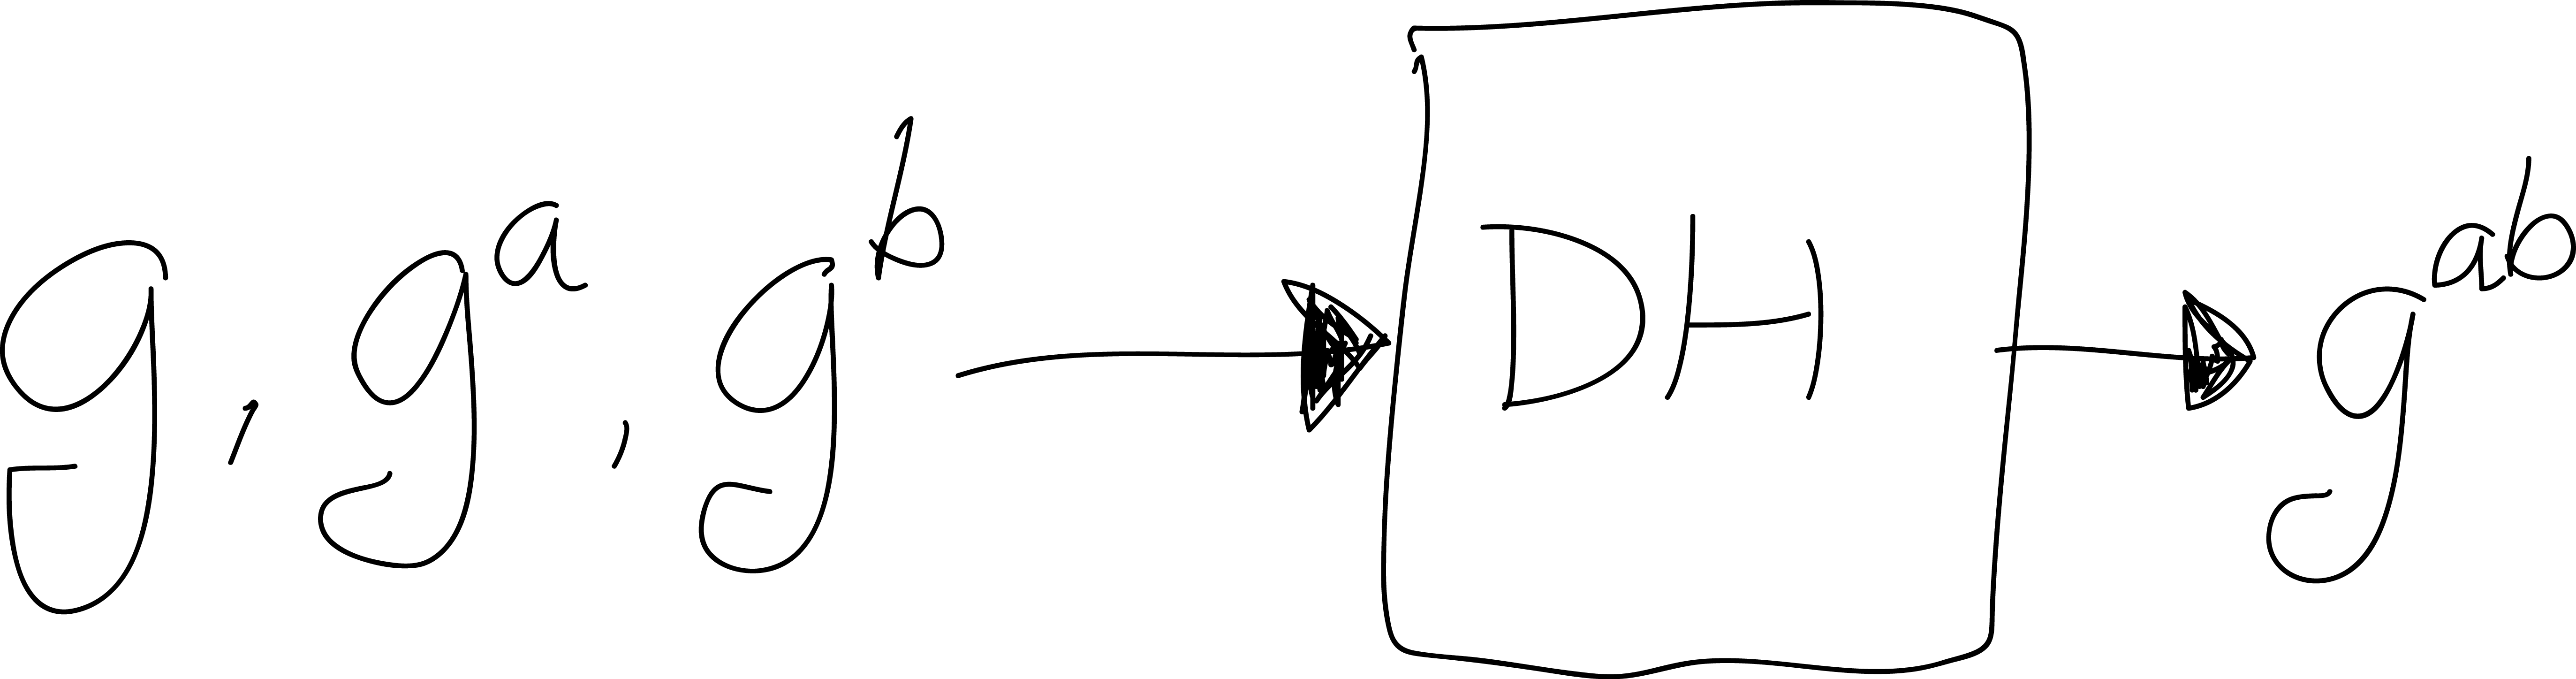
\includegraphics[width=60mm]{dh-oracle}
    \caption{Diffie Hellman oracle}
    \end{figure}
    
    \begin{subproblem}
  \begin{figure}
    \centering
    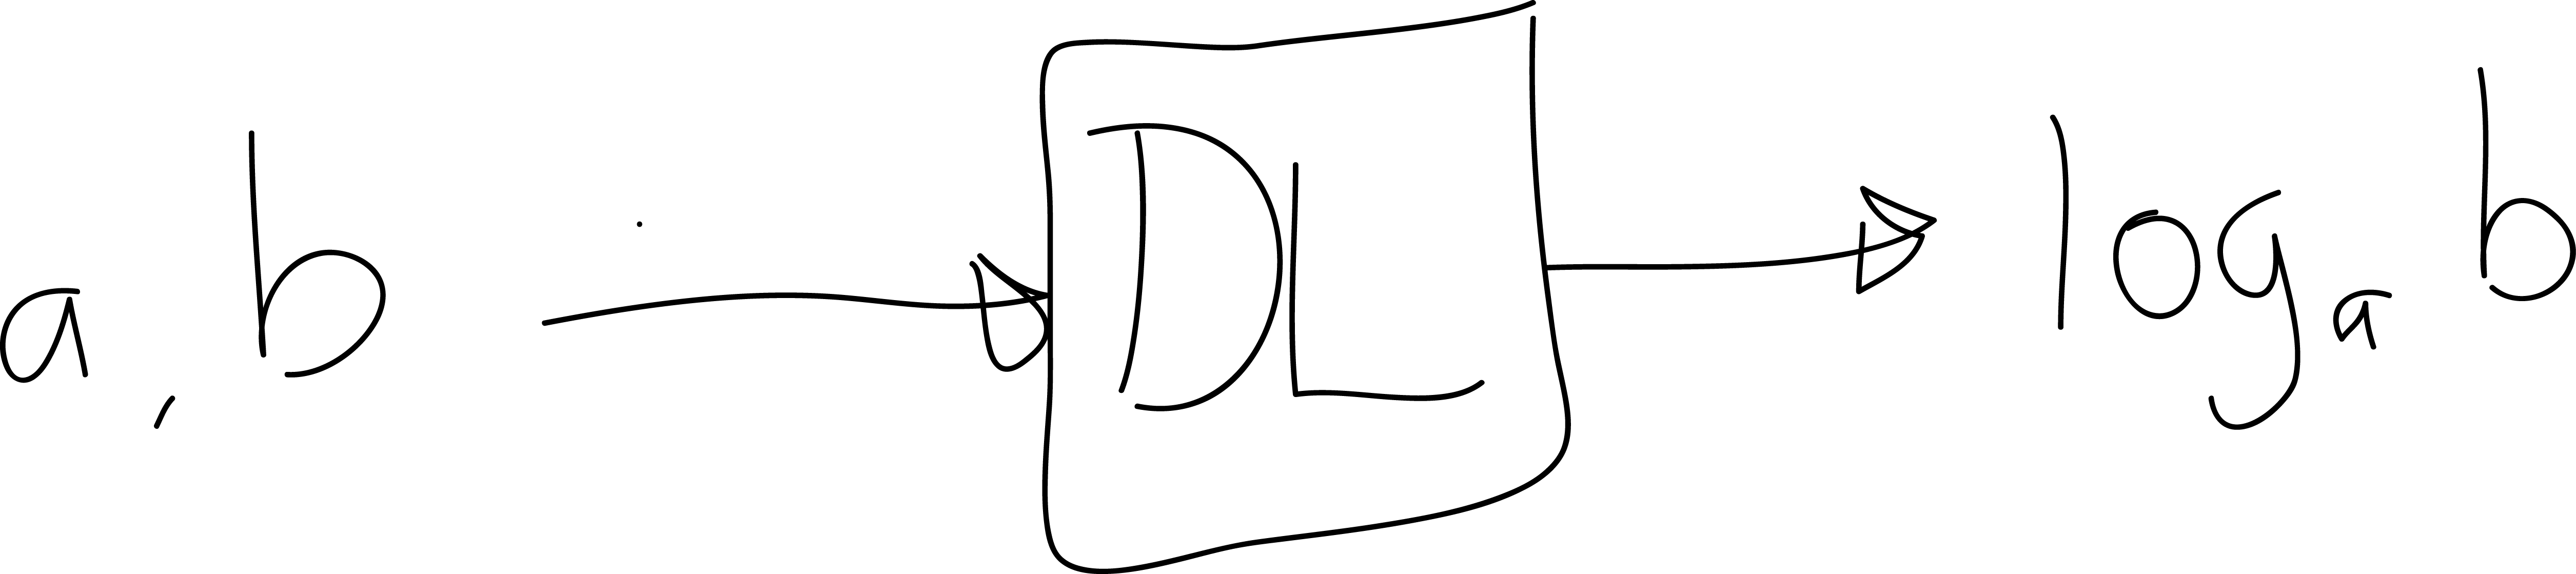
\includegraphics[width=60mm]{dl-oracle}
    \caption{Discrete Logarithm oracle}
    \end{figure}
    
    (2T) For the sake of conciseness: An oracle is ineffective if the difference between an algorithm guessing and any polynomial time algorithm which the oracle can use is negligible. 
    
    Given that the DH oracle is ineffective (i.e is guessing) we'll prove that the DL oracle is ineffective too. We can do this by reducing the DH problem to the DL problem.

      Reduction:
      \begin{verbatim}
      DH(g, g^a, g^b):
        a = DL(g, g^a)
        b = DL(g, g^b);
        return g^(ab);
    \end{verbatim}
    
Two calls to $D$L is required to extract $a$ and $b$. We can now calculate $g^(ab)$ effectively by using square and multiply twice (first calculate $g^a$ and then $(g^a)^b$. This can be done using $\log n$ multiplications, so the reduction is indeed polynomial. Thus, the DL problem must be at least as hard as the DH problem and if all DH oracle is ineffective, any DL oracle must be ineffective too.
    
     
  \end{subproblem}
  \begin{subproblem}
    (2T) % Prove that the DDH assumption implies the DH assumption.
    Reduction:
    \begin{verbatim}
    // answers yes iff c=ab
    DDH(g, g^a, g^b, c):
        g^ab=DH(g, g^a, g^b);
        g^c=modExp(g, c);
        if g^c==g^ab then 
          return YES;
        else 
          return NO;
    \end{verbatim}
    The only routine which takes more than constant time is modExp which goes in logarithmic time.
    We can reason in the same way as above to show that DH must be at least as hard as DDH and if any polynomial time algo for DDH is assumed to be negligable, then DH must be negligable too.
  \end{subproblem}
\end{problem}

\begin{problem}
  \begin{subproblem}
    (6T) % Describe an algorithm and perform a heuristic analysis of its expected running time.
%Implement your algorithm and compare your practical results with your theoretical analysis.
Tactics: Since the best way of generating a random prime is to choose a random number and look if it is a prime, I'll assume the same thing apply
if you want to generate a prime $p_{1}$ such that $p_{2}=\frac{p_{1}-1}{2}$ and $p_{3}=\frac{p_{2}-1}{2}$ are primes as well (Wikipedia also says there exists no special algorithm to find such primes, so it seems like my assumption is not that far fetched).
Let's call $p_{2}$ and $p_{3}$ Twin Sophie-Germain primes and $p_{1}$ its associated safe prime. If we assume the bias between $p_{1}$ and $p_{2}$ to be small, we could see it as we pick three random numbers that all have to be a prime. The probability of picking such numbers would be $\frac{2}{(n*\ln{2})^3}$ (if we only look at odd numbers). If we want to generate, say a 2048-bit prime $p_{1}$, we have to consider 720 million numbers before finding a safe prime with two Sophie-Germain primes. However, many candidates for $p_{2}$ and $p_{3}$ can be ruled out pretty fast since any Sophie-Germain prime must be congruent to $2$ modulo $3$. Thus the algorithm is as follows
\begin{enumerate}
\item Pick a random odd number $p_{1}$ consisting of $n$ bits.
\item Calculate $p_{2}=\frac{p_{1}-1}{2}$ and $p_{3}=\frac{p_{2}-1}{2}$.
\item If $p_{2} \neq 2 \mod 3$ then goto 1.
\item $p_{3} \neq 2 \mod 3$ then goto 1.
\item Run Miller-Rabbin or similar prime test on $p_{i}$, $1 \le i \le 3$. If one of the tests fail, then goto 1.
\item Return $p_{1}$.
\end{enumerate}
The algorithm turned out to be faster if you just skipped step 3 and 4, instead you can do only a few rounds Miller-Rabbin on $p_{2}$ and $p_{3}$ and if they both happen to look like primes you do another bunch of tests.

Model: Given that $p_{1}$ is a prime; how many random picks are expected to get $p_{2}$ and $p_{3}$ also primes? $f(\text{all three primes | } p_{1} \text{ prime}) = 0.5*(n*\ln{2})^2$ where $n$ is the number of bits in $p_{1}$.
Plot is in appendix 1.
\end{subproblem}
  \begin{subproblem}
    (2T) I ran some tests for Twin Sophie-Germain primes of bitlength 100 for different constants $2 \le c \le 10$. 
    Each test suite consisted of ten tests. I took the average from the number of picks required to find a Twin Sophie-Germain prime for each test suite. I could not see any increase/decrease in the number of tries required between different values on $c$. Plot is in appendix 2.
    
    Here is some sample code:
    
    \begin{verbatim}
    public SophieGermain() {
     System.out.println("f, avg(tries)");
      for (int f=2; f<=10; f++) {
        int sum = 0;
        for (int i=0; i<10; i++) {
        sum+=test(f, 100);
      }
      System.out.println(f + ", " + sum/10);
     }
    }
 
    // returns the number of tries before finding a 
    //twin sophie-germain prime with factor f
    private int test(int f, int b) {
     int t = 0;
     while (true) {
       t++;
       BigInteger p1 = BigInteger.probablePrime(b, r);

       BigInteger p2 = p1.subtract(BigInteger.ONE).
         divide(new BigInteger(String.valueOf(f)));
       if (!p2.isProbablePrime(3)) continue; // 0.875%

       BigInteger p3 = p2.subtract(BigInteger.ONE).
         divide(new BigInteger(String.valueOf(f)));
       if (!p3.isProbablePrime(3)) continue;

       if (!p2.isProbablePrime(64)) continue;
       if (!p3.isProbablePrime(64)) continue;

       return t;
      }
    }


    \end{verbatim}
  \end{subproblem}
\end{problem}


\begin{problem}
  (5T) NOT SOLVED % We leave this place holder here for improved readability.
\end{problem}

\begin{problem}
  \begin{subproblem}
    (7T) NOT SOLVED % We leave this place holder here for improved readability.
  \end{subproblem}
  \begin{subproblem}
    (3T) NOT SOLVED % We leave this place holder here for improved readability.
  \end{subproblem}
\end{problem}

\begin{problem}
  (2T) % Legendre/Jacobi symbol
  \begin{enumerate}
  \item $(26/97)=-1$ is a Legendre symbol because 97 is prime.
  \item $(17/995)=1$ is a Jacobi symbol because $995=5*199$ is composite.
  \item $(39/14)$ is not defined because 14 is even (I calculated it anyway and it turned out to be 1, but I suppose this is a bogus value).
  \item $(562045798654/754835)=-1$ is a Jacobi symbol because $754835=5*150967$ is composite.
  \item The last guy is undefined (last digit in denominator is a six, which is divisible by 2), and I don't want to calculate it.
  \end{enumerate}
  
  Calculations with intermediate steps are available on a separate piece of paper.
\end{problem}

\begin{figure}
    \centering
    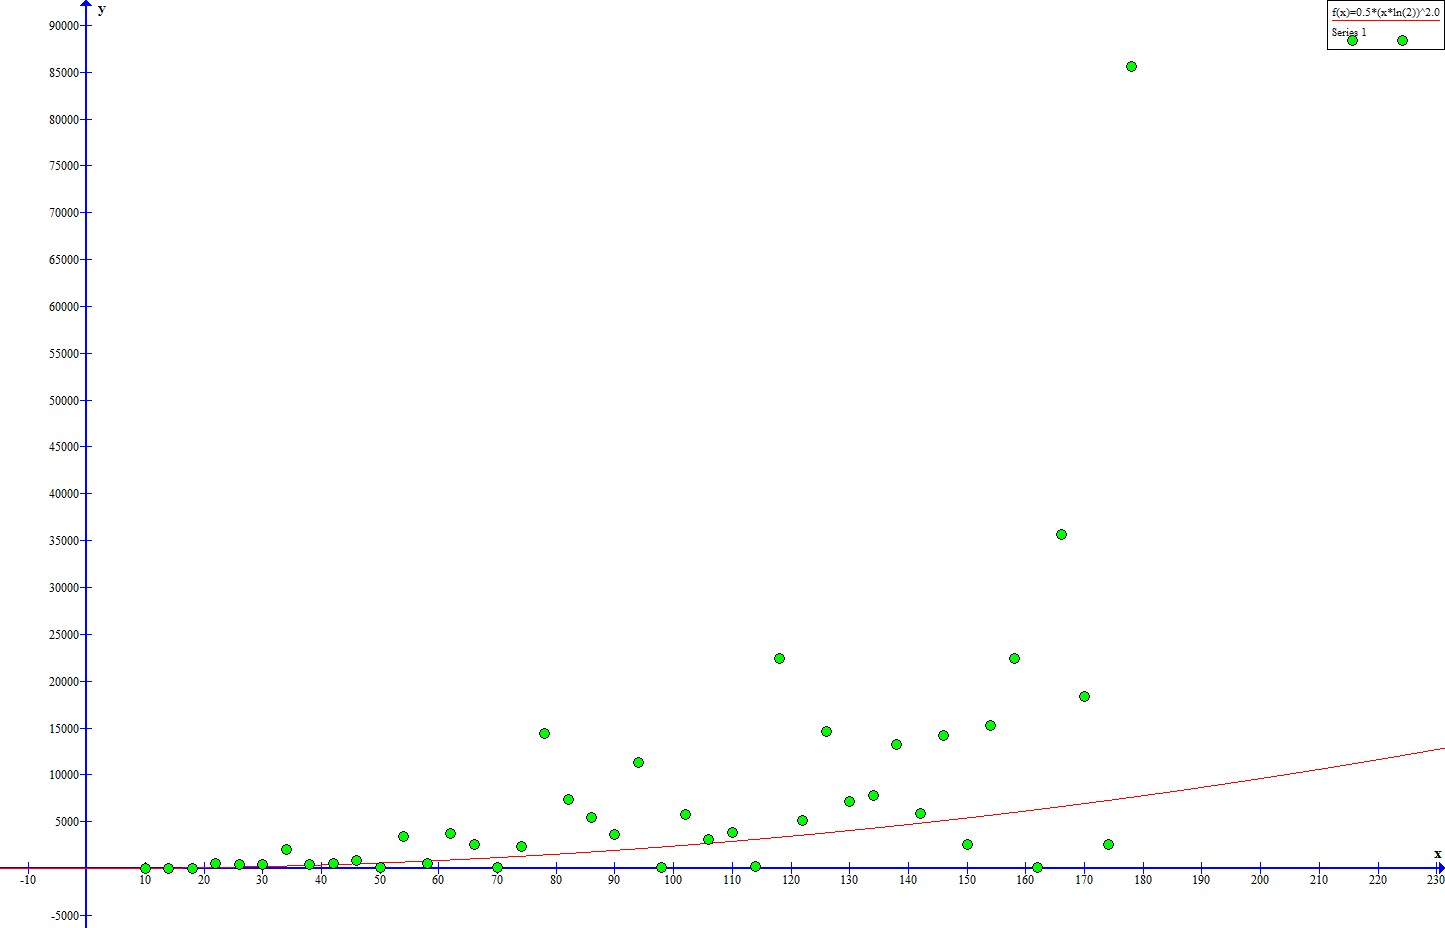
\includegraphics[angle=90, height=210mm]{sgt-primes}
    \caption{Number of bits on x-axis and iterations on y-axis.}
\end{figure}

\newpage
\begin{figure}
    \centering
    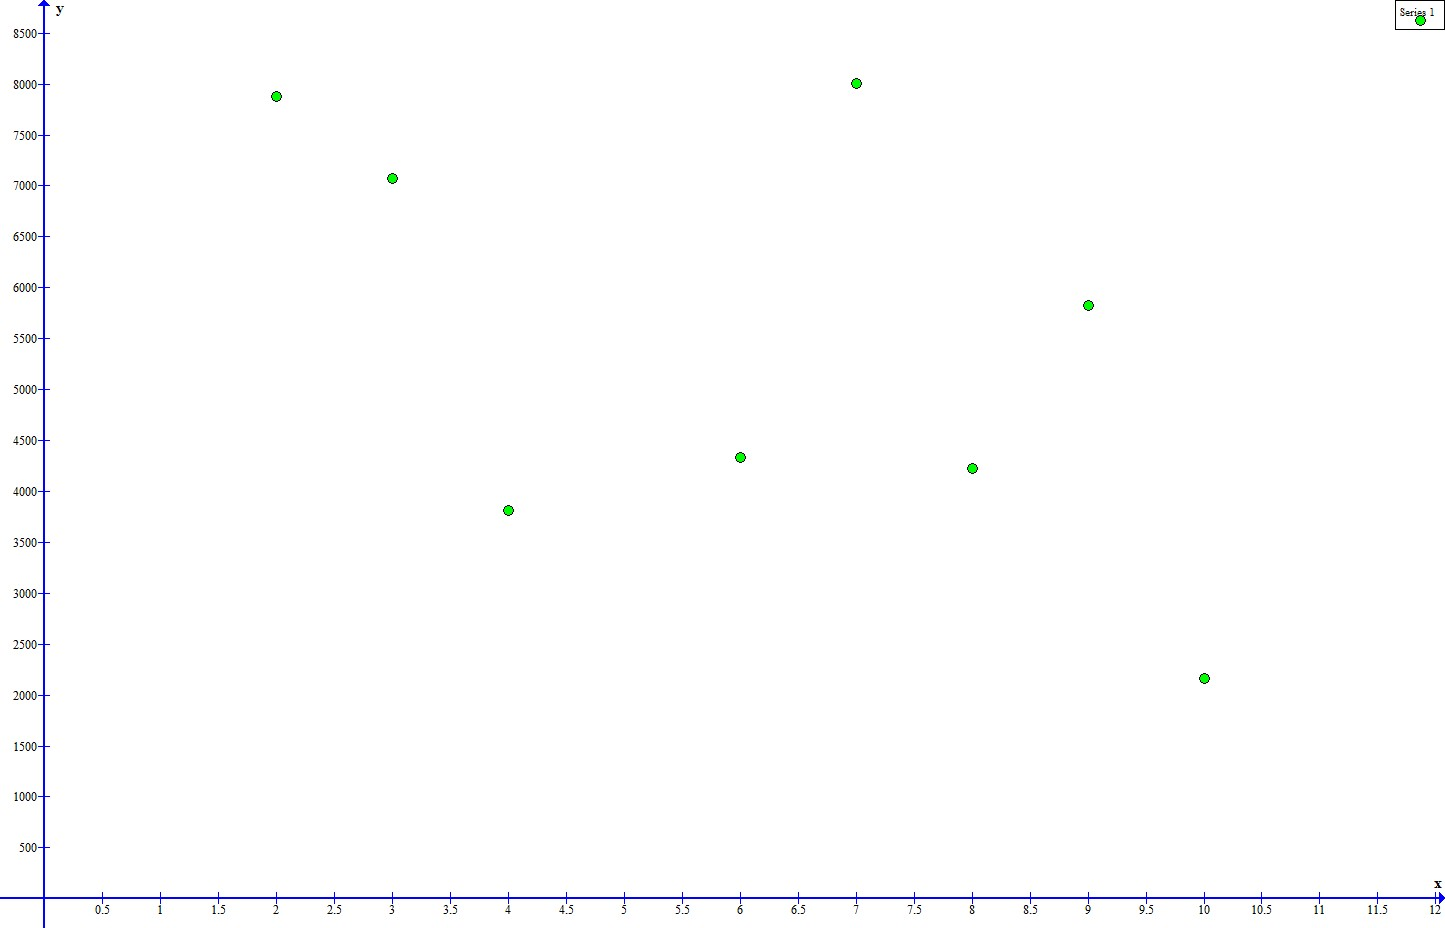
\includegraphics[angle=90, height=210mm]{sgt-factors}
    \caption{Factor $f$ in $p_{1}=fp_{2}+1$ on x-axis and iterations on y-axis. I know my test is very small, so perhaps that's the reason why you cannot see any pattern.}
\end{figure}

\end{document}
